\documentclass[12pt]{article}
\usepackage[margin=1in]{geometry}
\usepackage{graphicx}
\author{Tianyu Dai}
\title{PHY781 - Project 1}
\date{}
\begin{document}
\maketitle
\section*{1.}
The code of the Monte Carlo algorithm is attached in Appendix A. \\
In Fig. (1), the fluctuation of different number of steps in one block is shown. We can see that when , the fluctuation is smaller. However, the error of the data should not be influenced by the dividing of blocks. \\
\begin{figure}{\label{block}}
\centering
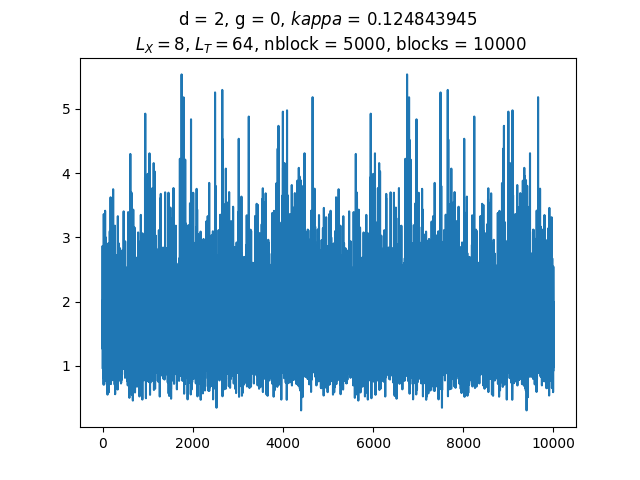
\includegraphics[width=0.6\textwidth]{2d_8-64_5000_10000.png}
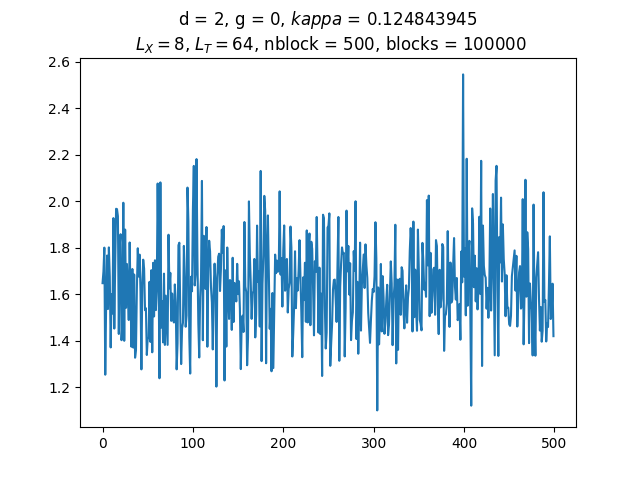
\includegraphics[width=0.6\textwidth]{2d_8-64_500_100000.png}
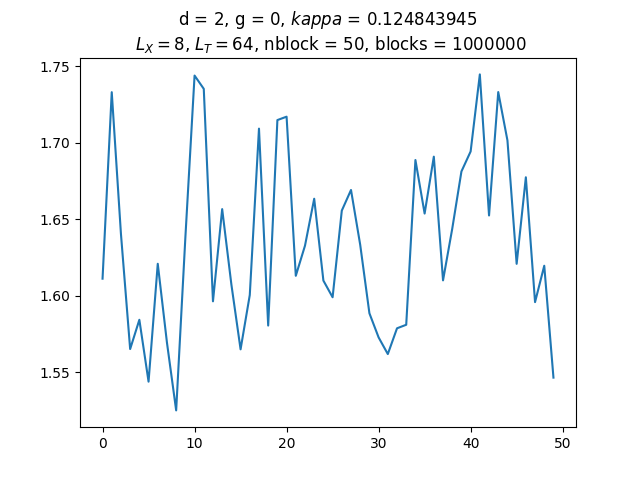
\includegraphics[width=0.6\textwidth]{2d_8-64_50_1000000.png}
\caption{Same data with different blocks. }
\end{figure}

\section*{2.}
\subsection*{(a)}
Assume $g=0$ for the following table. \\
Exact value of correlation function is calculated by computing the inverse matrix of M (code is attached in Appendix B). \\
\begin{center}
\begin{tabular}{|c|c|c|c|c|c|c|}
\hline 
d & $L_X$ & $L_T$ & $\kappa$ & \multicolumn{3}{c|}{$C_l^0$} \\ 
\hline 
\multicolumn{4}{|c|}{•} & Exact & Monte Carlo & Error\\ 
\hline 
2 & 8 & 48 & 0.249376559 & 3.6671260339 & 3.66489 & 0.015663\\ 
\hline 
2 & 8 & 64 & 0.249376559 & 1.6374308332 & 1.63529 & 0.00985065\\ 
\hline 
2 & 8 & 96 & 0.249376559 & 0.3302833014 & 0.336196 & 0.0063583537\\ 
\hline 
2 & 8 & 128 & 0.249376559 & 0.0667231504 & 0.0684529 & 0.000932522\\ 
\hline 
2 & 16 & 48 & 0.249376559 & 3.6671260339 & 3.66079 & 0.0148766\\ 
\hline 
2 & 16 & 64 & 0.249376559 & 1.6374308332 & 1.63408 & 0.0178285\\ 
\hline 
4 & 4 & 16 & 0.124843945 & 45.062275293 & 45.7849 & 1.00812\\ 
\hline 
4 & 8 & 16 & 0.124843945 & 45.062275293 & 44.3731 & 0.887142\\ 
\hline 
\end{tabular}
\end{center} 
\newpage

\subsection*{(b)}
Assume $g = 0.01$ for the following table. \\
\begin{center}
\begin{tabular}{|c|c|c|c|c|c|}
\hline 
d & $L_X$ & $L_T$ & $\kappa$ & \multicolumn{2}{c|}{$C_l^0$} \\ 
\hline 
\multicolumn{4}{|c|}{•} & Monte Carlo & Error\\ 
\hline 
2 & 8 & 16 & 0.249376559 & 0.0153983 & 4.81E-05\\ 
\hline 
2 & 8 & 20 & 0.249376559 & 0.00363053 & 1.67E-05\\ 
\hline 
2 & 8 & 24 & 0.249376559 & 0.000848118 & 6.04E-06\\ 
\hline 
2 & 8 & 32 & 0.249376559 & 4.77082E-05 & 7.36E-07\\ 
\hline 
2 & 16 & 16 & 0.249376559 & 0.0154688 & 3.02E-05\\ 
\hline 
2 & 16 & 20 & 0.249376559 & 0.00364392 & 1.06E-05\\ 
\hline 
2 & 16 & 24 & 0.249376559 & 0.00085015 & 2.95E-06\\ 
\hline 
2 & 16 & 32 & 0.249376559 & 4.74247E-05 & 2.10E-07\\ 
\hline 
4 & 4 & 16 & 0.124843945 & 0.0041509 & 4.12E-05\\ 
\hline 
4 & 8 & 16 & 0.124843945 & 0.00430892 & 4.19E-05\\ 
\hline 
\end{tabular} 
\end{center}

\section*{3.}
The data for $d = 2$ and $L_X = 8$ are fitted to the equation $C_0^l = A\exp(-M^l L_T/2)$. In the free case, $M^l = 0.1004761$, $A = 40.8477518$. As proven in Project 2 Problem 2, the correlation function exponentially decays as the time steps increase. However, when the coupling changes by a small amount, $M^l$ changes a lot. When $g = 0.01$, $M^l = 0.72286605$, and $A = 5.00007676$. $M_{phys}a = M^l$, $m_0a = \sqrt{1/\kappa-2d}$. We can see that in the free case, $M_{phys}$ and $m_0$ are similar. However, in the interacting case, $M_{phys}$ and $m_0$ have a large difference. \\
The fitting code is attached in Appendix B. \\
\end{document}
